
\section{Grammar}

This is the description of the Grammar class as it has been used for the general experimentations that can be found in the chapter 3.
A more efficient version that can handle linear and Chomsky normal-form grammars has been implemented and is presented later in this report.

The different productions of the context-free grammar are given by the user through a file following the same pattern as the example of section 1.1.2.
\\
\\
The program uses the following conventions:
\begin{itemize}
    \item[$-$] Every \textit{non-terminal} is a single uppercase letter.
    \item[$-$] Every \textit{terminal} is a single other ASCII character.
    \item[$-$] The right-hand is composed of one or several groups, each group is either a pair of \textit{non-terminals} or a single \textit{terminal}.
\end{itemize}

When the program comes accross an uppercase letter it automaticly transorms it into an index beginning from 0, so 'A' becomes 0, 'B' becomes 1, etc.
\\
\\
My program then fills three variables:
\begin{itemize}
    \item[$-$] The variable `non\_terminals' is a string, when a new \textit{non-terminal} is read from the file it is converted as described above and then added as a character to the variable. This variable will then make it easy and efficient to access the rules.
    \item[$-$] The variable `non\_terminal\_rules' is a three dimensional array of integers.
        \begin{enumerate}
            \item The first dimension has the size of the latin alphabet: 26, each line of this dimension will allow access to the non-terminal rules of the corresponding \textit{non-terminal}, using the converted values stored in `non\_terminals'.
            \item The second dimension allows access to the different pairs of \textit{non-terminals}.
            \item The third dimension has a size of 2, it represents the pair of \textit{non-terminals}.
        \end{enumerate}
    \item[$-$] The variable `terminal\_rules' is a two dimensional array of integers.
        \begin{enumerate}
        \item The first dimension has the size of the latin alphabet, each line of this dimension allows access to the terminal rules of the corresponding \textit{non-terminal}.
        \item The second dimension allows access to the different \textit{terminals} related to that \textit{non-terminal}.
        \end{enumerate}
\end{itemize}

The point of seperating the \textit{non-terminal} rules from the \textit{terminal} ones in two variables is that they are always accessed on different cases. It would then slow down the processus to always have to differenciate them from one another.

\section{Naive parser}

The naive implementation uses the divide and conquer approach, 

\FloatBarrier
\begin{algorithm}
    \caption{Naive parser}
    \label{parse}
    \begin{algorithmic}[1]
        \State $s \gets input\_string$
        \Procedure{parse}{$var, i, j$} \Comment{Recursive parser function}
            \If{$i == j - 1$}
                \ForAll{$t \in terminal\_rule[var]$}
                    \If{$t == s[i]$}
                        \State \textbf{return} $true$
                    \EndIf
                \EndFor
            \Else
                \ForAll{$nt \in non\_termial\_rules[var]$}
                    \For{$k \gets i + 1; k < j$}
                        \If{$parse(nt[0], i, k) \land parse(nt[1], k, j)$}
                            \State \textbf{return} $true$ 
                        \EndIf
                    \EndFor
                \EndFor
            \EndIf
            \State \textbf{return} $false$
        \EndProcedure
    \end{algorithmic}
\end{algorithm}
\FloatBarrier

\subsection{Complexity of the algorithm}

To find the complexity of this algorithm one can draw recursion trees for small values of $n$ and find the following sequence: $0, 2, 8, 26, 80$\dots
After some research it is possible to find out that this sequence corresponds to the formula $3^{n - 1} - 1$ \cite{naive_formula}.

The resulting complexity of this algorithm is then $O(3^n)$.

\section{Top-down parser}

The top-down implementation is almost the same as the naive one, except that there is here a global variable that memorize every computed results.

\FloatBarrier
\begin{algorithm}
    \caption{Top-down parser}
    \label{parse}
    \begin{algorithmic}[1]
        \State $table$ is a 3d array of 0
        \State $s \gets input\_string$
        \Procedure{parse}{$var, i, j$} \Comment{Recursive parser function}
            \If{$table[var, i, j] != 0$}
                \State \textbf{return} $(table[var, i, j] == 1)$
            \EndIf
            \If{$i == j - 1$}
                \ForAll{$t \in terminal\_rule[var]$}
                    \If{$t == s[i]$}
                        \State $table[var, i, j] \gets 1$
                        \State \textbf{return} $true$
                    \EndIf
                \EndFor
            \Else
                \ForAll{$nt \in non\_terminal\_rules[var]$}
                    \For{$k \gets i + 1; k < j$}
                        \If{$parse(nt[0], i, k) \land parse(nt[1], k, j)$}
                            \State $table[var, i, j] \gets 1$
                            \State \textbf{return} $true$ 
                        \EndIf
                    \EndFor
                \EndFor
            \EndIf
            \State $table[var, i, j] \gets 2$
            \State \textbf{return} $false$
        \EndProcedure
    \end{algorithmic}
\end{algorithm}
\FloatBarrier

\subsection{Complexity of the algorithm}

To compute the running-time of the top-down algorithm we can count the number of cells in the memoization table and multiply it by the complexity of the inner loops of the algorithm.
This will give an upper bound of the complexity.
The loops that go through the grammar are ignored, the size of the table is $n^2$, with $n$ the size of the input string, the complexity of the parse function without any recursion is $O(n)$, so the complexity of the top-down parser is $O(n * n^2) = O(n^3)$.

\section{Bottom-up parser}

For this parser there are two possible implementation versions, one uses a boolean table and the other one uses a string table, their process are slightly different and they give different results in term of iterations and running time.

In the first approach the goal is to complete a triangular matrix, when the matrix is fully completed it watches the last cell and if it finds the \textit{start symbol} in it it returns true, otherwise it returns false.
That version is called the `string' bottom-up parser in this report.

\FloatBarrier
\begin{algorithm}
    \caption{`String' bottom-up parser}
    \label{parse}
    \begin{algorithmic}[1]
        \Procedure{parse}{$s$} \Comment{Iterative parser function}
            \State $matrix$ is a 2d array of empty strings
            \State $step \gets 0$
            \For{$i \gets 0; i < s.length()$}
                \ForAll{$var \in non\_terminals$}
                    \ForAll{$t \in terminal\_rules[var]$}
                        \If{$t == s[i]$}
                            \State Add $var$ to $matrix[step, i]$ if not already inside
                        \EndIf
                    \EndFor
                \EndFor
            \EndFor
            \State $step \gets step + 1$
            \While{$s.length() - step > 0$}
                \For{$i \gets 0; i < s.length() - step$}
                    \For{$j \gets 0; j < step$}
                        \State $r \gets check\_combs(matrix[j, i], matrix[step - (j + 1), i + j + 1])$
                        \State Add $r$ to $matrix[step, i]$ if not already inside
                    \EndFor
                \EndFor
                \State $step \gets step + 1$
            \EndWhile
            \State \textbf{return} is the start symbol in $matrix[s.length() - 1, 0]$ ?
        \EndProcedure
        \Procedure{check\_combs}{$cell\_1, cell\_2$}
            \State $result$ is an empty string
            \For{$i \gets 0; i < cell\_1.length()$}
                \For{$j \gets 0; j < cell\_2.length()$}
                    \State $production \gets cell\_1[i] . cell\_2[j]$
                    \If{$production$ is in the $non-terminal\_rules$}
                        \State Add the left hand of the matching rule to $result$
                    \EndIf
                \EndFor
            \EndFor
            \State \textbf{return} $result$
        \EndProcedure
    \end{algorithmic}
\end{algorithm}
\FloatBarrier

In the second approach the goal is to complete a boolean table, then it looks in a specific cell and returns the result.
That parser is called the `boolean' bottom-up parser in this report.

\FloatBarrier
\begin{algorithm}
    \caption{`Boolean' bottom-up parser}
    \label{parse}
    \begin{algorithmic}[1]
        \Procedure{parse}{$s$} \Comment{Iterative parser function}
            \State $matrix$ is a 3d array of false booleans
            \State $step \gets 0$
            \For{$i \gets 0; i < s.length()$}
                \ForAll{$var \in non\_terminals$}
                    \ForAll{$t \in terminal\_rules[var]$}
                        \If{$t == s[i]$}
                            \State $matrix[0, i, var] \gets true$
                        \EndIf
                    \EndFor
                \EndFor
            \EndFor
            \State $step \gets step + 1$
            \While{$s.length() - step > 0$}
                \For{$i \gets 0; i < s.length() - step$}
                    \For{$j \gets 0; j < step$}
                        \ForAll{$var \in non\_terminals$}
                            \ForAll{$t \in terminal\_rules[var]$}
                                \State $bool\_1 \gets matrix[j, i, t[0]]$
                                \State $bool\_2 \gets matrix[step - j - 1, i + j + 1, t[1]]$
                                \If{$bool\_1 \land bool\_2$}
                                    \State $matrix[step, i, var] \gets true$
                                \EndIf
                            \EndFor
                        \EndFor
                    \EndFor
                \EndFor
                \State $step \gets step + 1$
            \EndWhile
            \State \textbf{return} $matrix[s.length() - 1, 0, start\_symbol\_index]$
        \EndProcedure
    \end{algorithmic}
\end{algorithm}
\FloatBarrier

The `boolean' implementation needs a predictable amount of iterations for a given grammar to parse a string, no matter what pattern this string follows.
The `string' one on the other hand needs a various number of iterations depending on the pattern of the input string.

\subsection{Complexity of the algorithms}

The two algorithms above have the same complexity, to determine it it is needed to look at the inner loops of the algorithms.
For both of them if the grammar loops are ignored the complexity is $O(n + n^3) = O(n^3)$.

\subsection{Expression of the number of iterations}

For the `boolean' bottom-up parser it is possible to predict the exact number of iterations that it will compute, indeed unlike the naive and top-down versions there is no recursion that denies us to anticipate it.

It is possible to translate the `for' and `while' loops into a mathematical expression:
\begin{equation} \label{eq:bottom-up_iterations_with_sum}
    iterations = n \cdot gt + \sum_{k = 1}^n (n - k) \cdot k \cdot gnt
\end{equation}

With:
\begin{itemize}
    \item[$-$] $n$ being the size of the input string.
    \item[$-$] $gt$ being the number of terminal rules: the number of \textit{terminals} on the right-hands of the grammar.
    \item[$-$] $gnt$ being the number of non terminal rules: the number of \textit{non-terminals} pairs on the right-hands of the grammar.
\end{itemize}

With such an expression it will be easier to justify the observed results in the `boolean' bottom-up parser case.

But the equation \ref{eq:bottom-up_iterations_with_sum} has an issue, it is not a polynomial function, which denies one from displaying it in a plot for example.
To get a real mathematical expression it is possible to use the Faulhaber's formulas that allows one to translate a sum into a polinomial function:

\begin{align*}
    iterations &= n \cdot gt + \sum_{k = 1}^n (n - k) \cdot k \cdot gnt\\
    &\Leftrightarrow n \cdot gt + gnt \cdot \sum_{k = 1}^n n \cdot k - k^2\\
    &\Leftrightarrow n \cdot gt + gnt \cdot (n \cdot \sum_{k = 1}^n k - \sum_{k = 1}^n k^2)\\
    &\Leftrightarrow n \cdot gt + gnt \cdot (\dfrac{n^2 \cdot (n + 1)}{2} - \dfrac{n \cdot (n + 1) \cdot (2 \cdot n + 1)}{6})
\end{align*}

The final expression is the following:
\begin{equation} \label{eq:bottom-up_iterations}
    iterations = n \cdot gt + \dfrac{gnt}{6} \cdot (3 \cdot n^2 \cdot (n + 1) - n \cdot (n + 1) \cdot (2 \cdot n + 1))
\end{equation}

The function above is a general expression of the number of iterations that the boolean bottom-up parser will have to do in order to parse a string of size $n$ for a grammar possessing $gt$ \textit{terminals} and $gnt$ pairs of \textit{non-terminals} on its right-hands.

With such function one can represent the behaviour of the number of iterations when the number of \textit{non-terminals} $gnt$ increases and the strings sizes $n$ too.

\FloatBarrier
\begin{figure}[h]
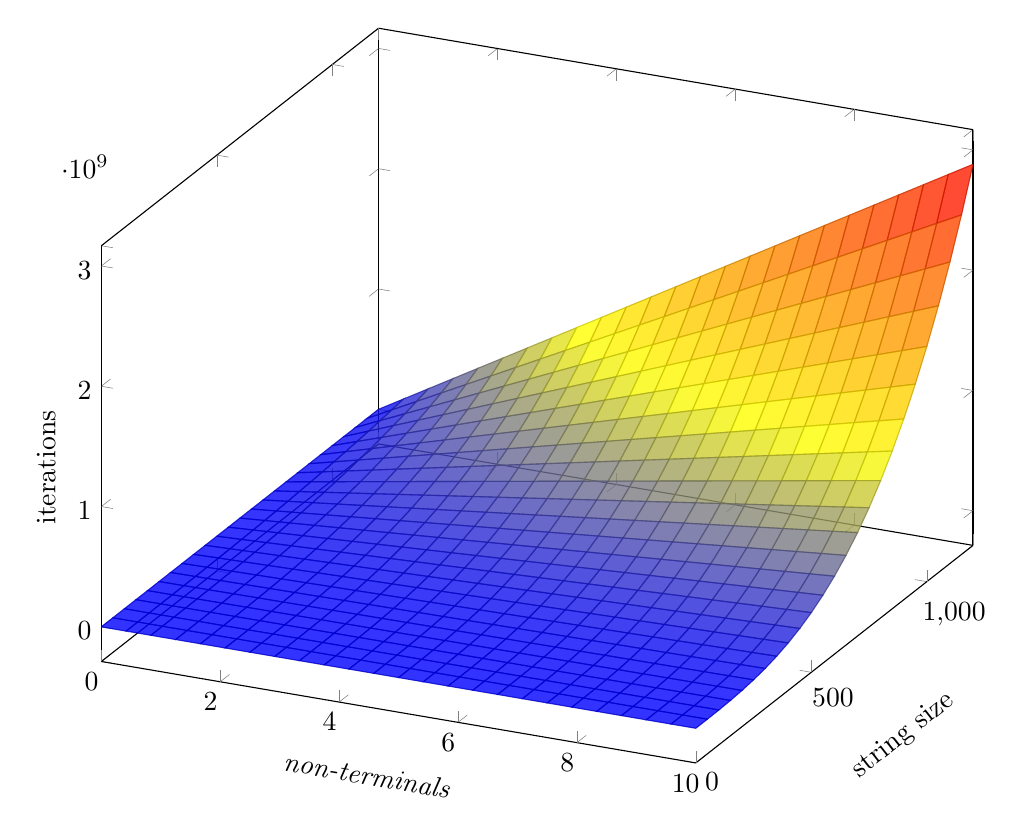
\begin{tikzpicture}
\begin{axis}[
    xlabel=\textit{non-terminals},
    ylabel=string size,
    zlabel=iterations,
    xlabel style={sloped like x axis},
    ylabel style={sloped},
    height=0.9\textwidth
]
\addplot3[
    surf,
    opacity=0.8,
    samples=25, samples y=25,
    domain=0:10,domain y=0:1200
]
    {y*0 + ((x/6) * (3*y*y*(y+1) - (y*(y+1)*(2*y+1))))};
\end{axis}
\end{tikzpicture}
\caption{3D plot of the function \ref{eq:bottom-up_iterations}}
\end{figure}
\FloatBarrier

It is interesting to see on the 3d plot that for a fixed $gnt$ when $n$ increases the number of iterations increases following a power function which should be of the form $y = a \cdot x^3$, since the complexity of the bottom-up parser is $O(n^3)$.

On the other hand when $n$ is fixed and that $gnt$ increases the number of iterations increases following a linear function.
That can be explained by the fact that the \textit{non-terminals} represent only on loop in the parser, so if the amount of \textit{non-terminals} is changed the impact on the number of iterations is linear.

